\documentclass[12pt,a4paper]{article}
\usepackage[czech]{babel}
\usepackage[utf8]{inputenc}
\usepackage[colorlinks=true]{hyperref} % Aktivní odkazy
\usepackage{graphicx} %vkládání obrázků
\usepackage{authblk} %Formátování autorů
\usepackage[backend=biber, style=iso-numeric, giveninits=true, maxbibnames=99]{biblatex} %spravuje interakci s literaturou, nastavuje ISO 690

\DeclareNameAlias{default}{last-first} %Formátování jmen v citacích
\makeatletter
\renewcommand\Authands{, } % Formátování autorů pro češtinu
\makeatother

\textwidth 15,92cm \textheight 24.62cm
\topmargin -2.2cm 
\oddsidemargin 0cm \evensidemargin 0cm

\pagestyle{empty}
\addbibresource{refs.bib}
\nocite{*} % Vytiskne celý .bib soubor bez nutnosti citovat

\title{Dálkové měření vzdálenosti pomocí laserového paprsku (LIDAR)}


\author[1]{Jakub Skalka}
\author[2]{Filip Landr}
\author[3]{Jaroslav Kraft}

\date{\small Garant: Ing. Kryštof Kadlec, KLFF FJFI\vspace{-2em}} % It is what it is. Je 16. 6. 9:00, je to šité horkou jehlou. \vspace je důležitý, jinak si budete krást místo pro příspěvek. Vždy musí být u posledního autora

\affil[1]{Gymnázium, České Budějovice, Jírovcova 8; skalkaj@jirovcovka.net}
\affil[2]{Gymnázium, Praha 5, Nad Kavalírkou 100/1; fi.landr@seznam.cz}
\affil[3]{ Ten třetí človíček\vspace{-1em}} %Ditto, \vspace musí být u posledního autora

\begin{document}

\maketitle \thispagestyle{empty}

\begin{abstract} \noindent
    Náš příspěvek se zaměřuje na aplikaci technologie dálkového měření vzdálenosti - LIDAR (Light Detection And Ranging). Tato technika je založena na stanovení doby šíření laserového paprsku odraženého od snímaného objektu. \\Věnuje se také základům generace laserového záření a měření výstupních parametrů u Q-spínaného mikročipového laseru Nd:YAG.\end{abstract}


\section{Úvod}
Úvodní a základní informace (motivace, současný stav problému, teoretický předpoklad)

\pagebreak
\section{Popis našeho laseru}
Při našem pokusu jsme použili mikročipový pasivně Q-spínaný laser Nd:YAG/V:YAG, který vyzařoval ve spektrální oblasti $1,3$ $\mu$m, která je “eyesafe”, tedy bezpečná pro lidské oko. Náš laser měl tvar válce s průměrem $5$ mm a délka aktivního prostředí Nd:YAG byly $4$ mm a délka saturovatelného absorbéru V:YAG byla $0,7$ mm. počáteční transmise absorbéru byla $85$ \% a reflektivita výstupního zrcadla byla $90$ \% v již zmiňované spektrální oblasti. Koncentrace iontů Nd$^{3+}$ v YAG matrici bylo 1,1 \% Nd/Y. 
\\Náš pevnolátkový laser byl čerpán laserovou diodou na vlnové délce 808 nm, která už není oku bezpečná. Dioda byla použita v pulsním režimu s délkou impulsu 500 um a opakovací frekvencí 50Hz. Proud na diodě byl nastaven na 30 A a teplota byla 30 °C. Pro zefektivnění čerpání, byla dioda navedena optickým vláknem do fokusační optiky, tvořenou kolimátorem a fokusační čočkou.

\section{Postup měření}
Měření probíhalo tak, že jsme si nastavili překážku pro laser v dané vzdálenosti a pustili laser aparaturou na obrázku, následně na osciloskopu našli graf laserového výboje který do fotodiody (záznamového zařízení) přišel přímo z rozdělovače záření a druhý “peak” který se odrazil od překážky. Pak jsme je porovnali na osciloskopu a ten nám udal čas mezi vlnami a tím pádem nám dal potřebnou informaci pro změření vzdálenosti mezi rozdělovačem a zábranou. Vzdálenost jsme vypočítali pomocí tohoto vzorečku (c*t)/2, díky kterému jsme dostali relativně přesné hodnoty s odchylkou měření do 60 cm, protože jeden pulz laseru měl délku 60 cm, kdybychom pulzy dělali kratší, tak budeme mít vyšší přesnost, ale pro naše podmínky a zadání tato přesnost stačila

\begin{figure}[bh]
    \centering
    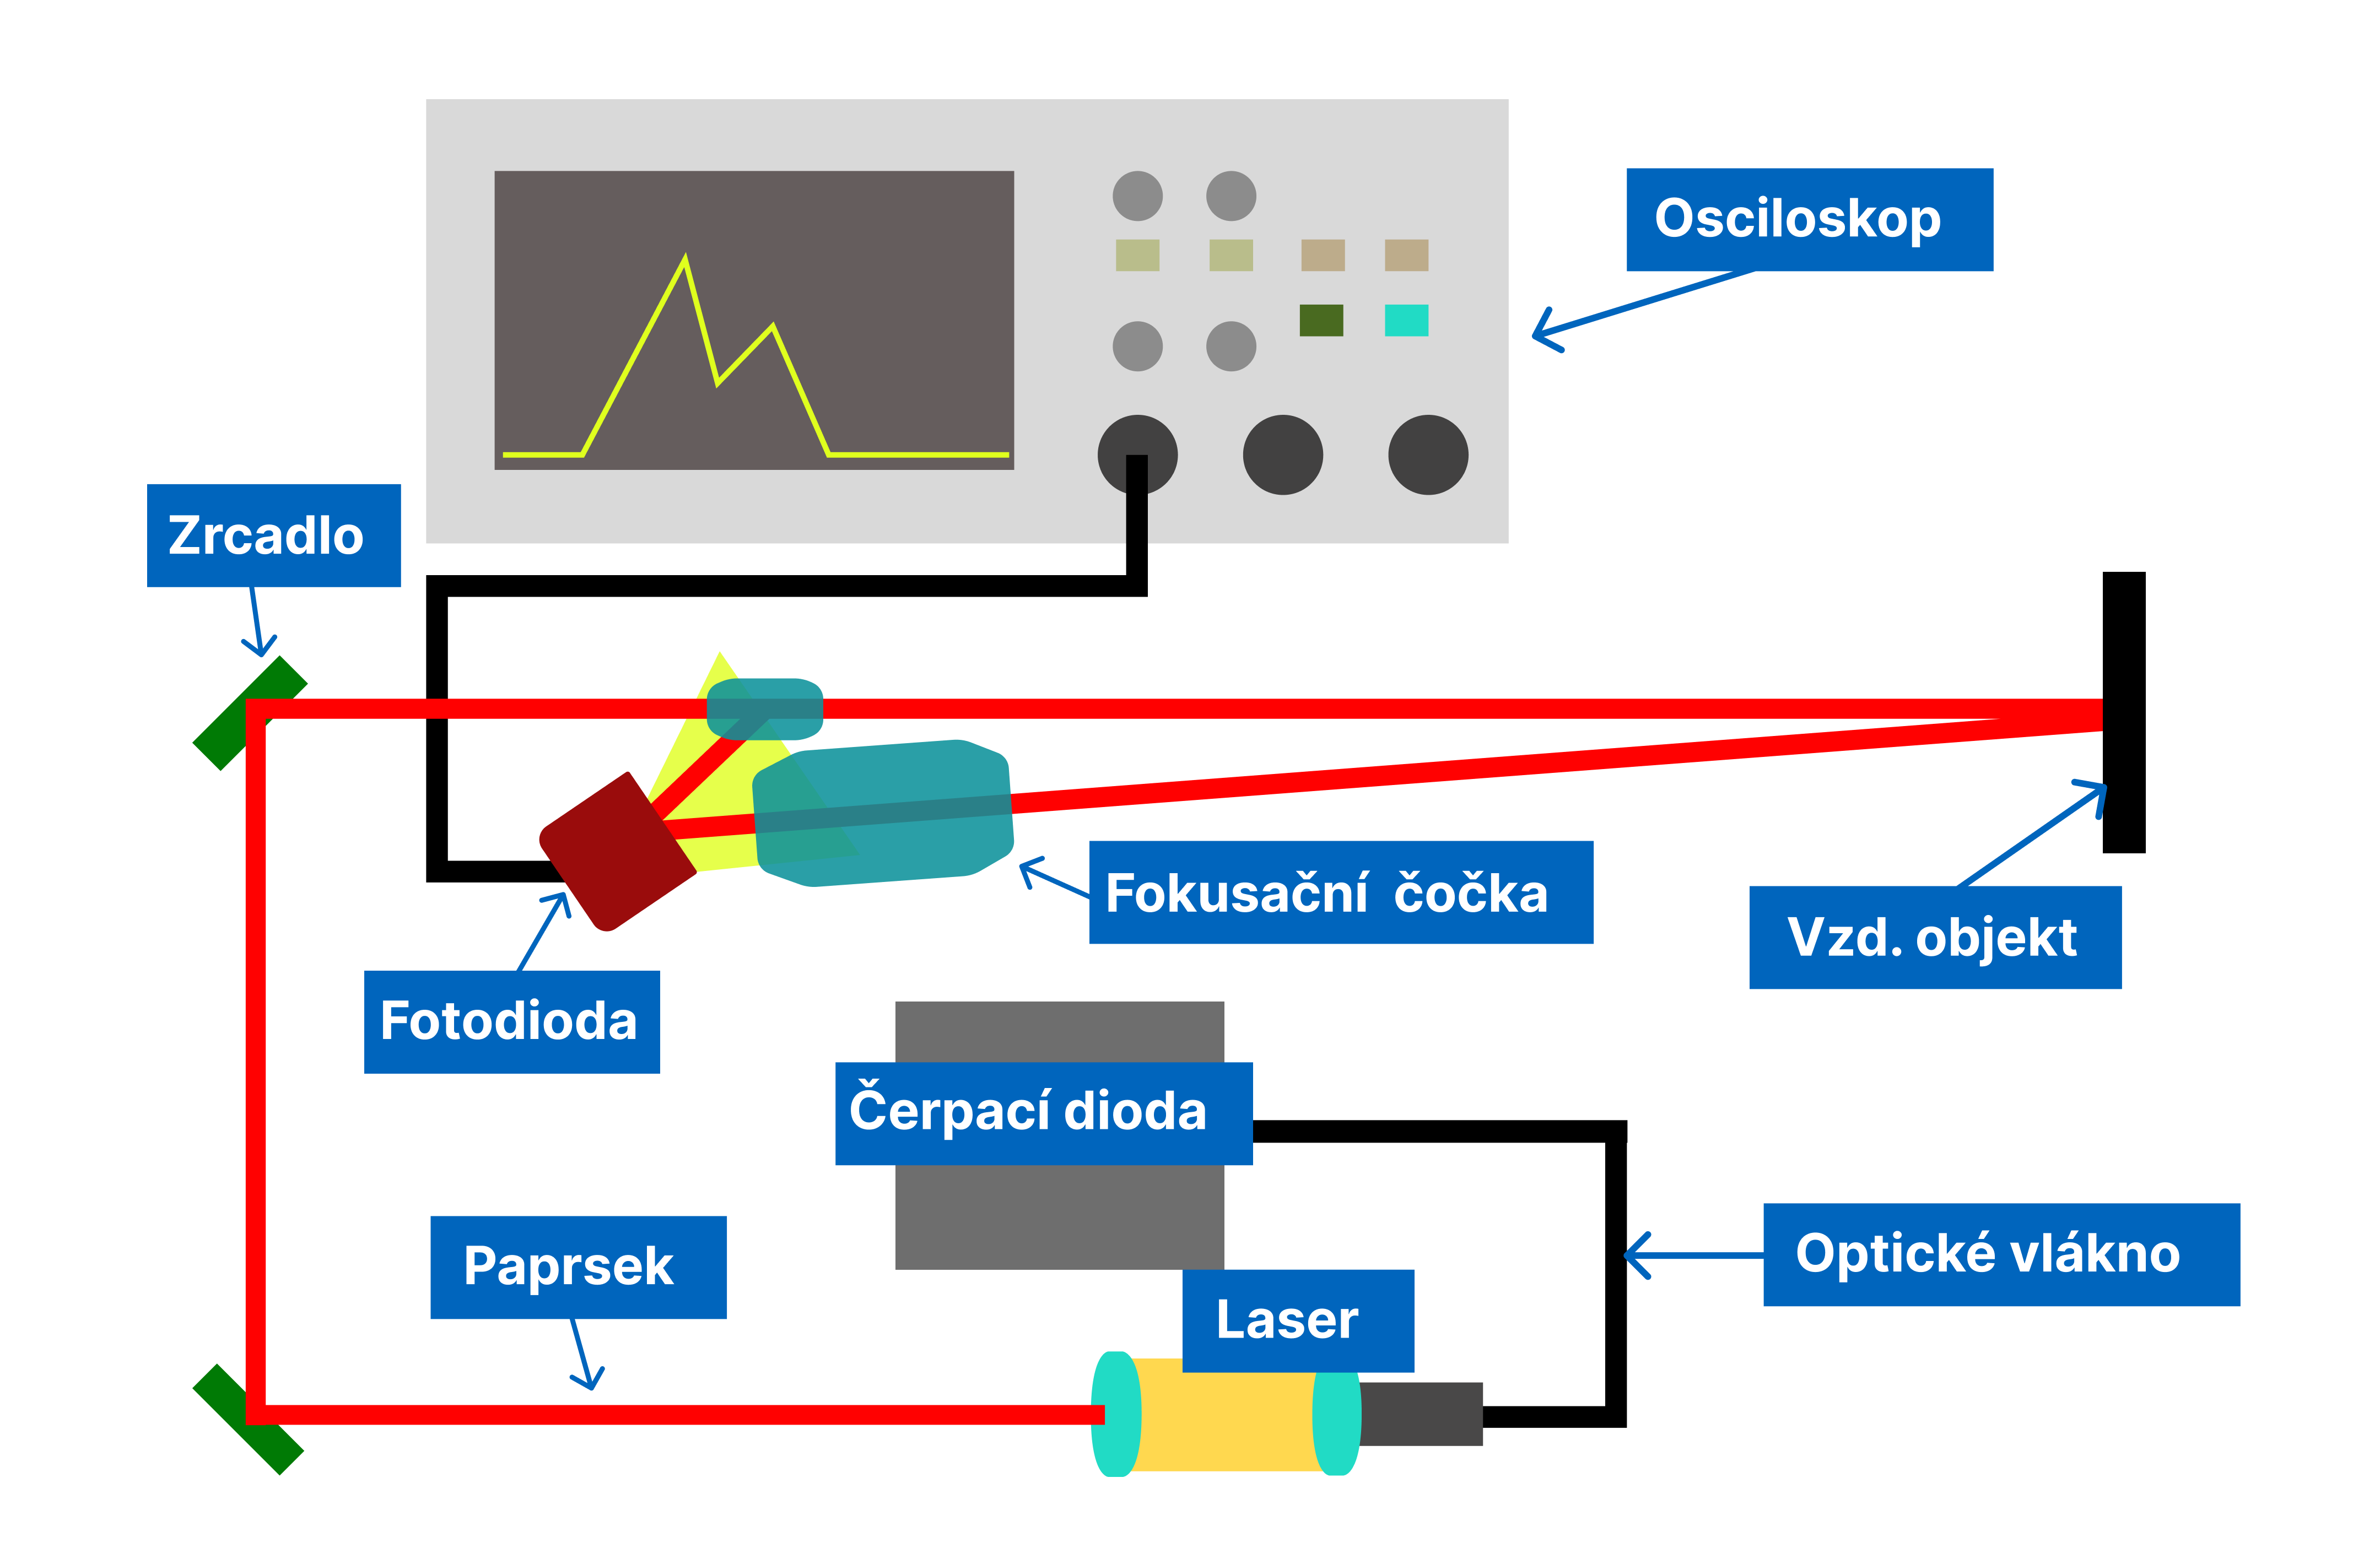
\includegraphics[width=0.5\textwidth]{Diagram měření.png}
    \caption{diagram měřící aparatury}
\end{figure}

\section{Výsledek měření}
Lorem Ipsum

\section{Shrnutí}
Závěrečné informace, shrnutí, vypíchnutí hledání, zodpovězení otázek, které motivovaly zkoumání, výhled do budoucna.



\section*{Poděkování}
Chtěli bychom velice poděkovat Ing. Kryštofovi Kadlecovi za jeho pomoc a podporu při vytváření tohoto příspěvku.
Náš dík patří také FJFI za umožnění výzkumu v rámci projektu a KLFF za poskytnutí prostoru.
\printbibliography

\end{document}